
\section{Experiments}

\subsection{Labor market moments}

\begin{figure}[t]
\begin{center}
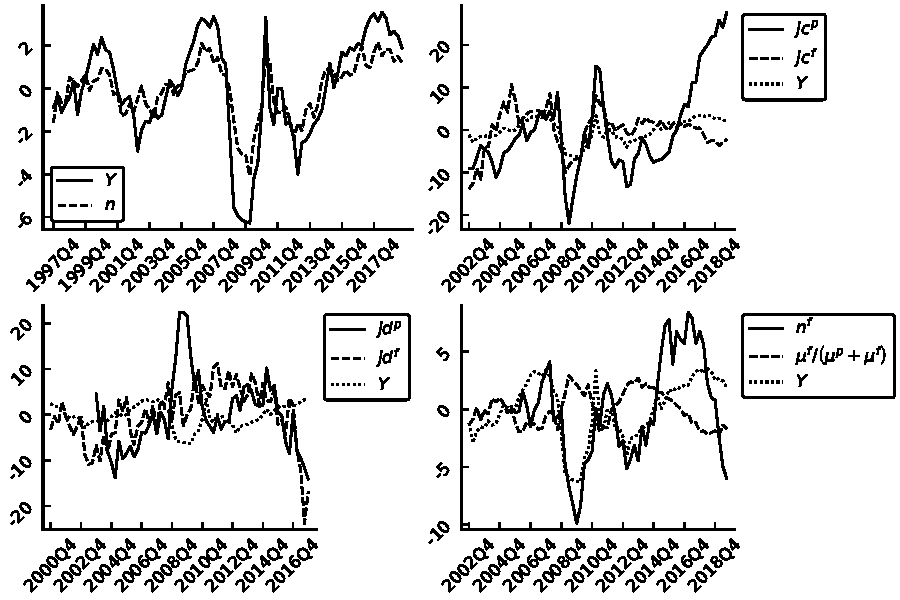
\includegraphics[scale=1.]{lm_moments.pdf}
\caption{Fluctuations in labor market values.}
\label{fluctuations}
\end{center}
\end{figure}

In this paragraph, we assess the ability of the model with respect to the reproduction of labor market moments. The absence of proper series for the computation of the latter in the Euro area represents a significant obstacle. As a result, I use series draws from French data as a proxy to account for the main features of a dual labor market.

The series are logged and filtered along the lines of \citet{hamilton2018you}. Importantly, I do not use the so-called Hodrick-Prescott filter, whether it be one-sided or two-sided. Indeed, \citet{hamilton2018you} explains the purely artifical statistical properties of series filtered through the Hodrick-Prescott method. The use of the Hodrick-Prescott filter imposes strong statistical properties on series because of its inner structure, regardless the process behind the actual data. Stunningly, when considering random walks, the output of the Hodrick-Prescott filter presents persistence. This behavior of the Hodrick-Prescott filter is all the more worrying since macroeconomic time series often boil down to martingales, whose increments remain unpredictable by definition. In standard macroeconomic samples of data, a band pass filter only captures the frequencies belonging to cycles with periodicity between 5 and 40 quarters. Considering growth rates exaggerates the high frequency margin in the data. Overall, a filtering method remains an arbitrary choice with many pitfalls\footnote{See \citet{gorodnichenko2010estimation}, \citet{ferroni2011trend}, \citet{lafourcade2012taking}, \citet{canova2014bridging} and \citet{hamilton2018you} for thorough developments of this idea}.

\begin{table}[H]
\begin{center}
\begin{tabular}{ccccc}
\toprule
 Variables & \multicolumn{2}{c}{Data} & \multicolumn{2}{c}{Model} \\ \cmidrule(lr){2-3} \cmidrule(lr){4-5} & Std. Dev. & $Cor\left( Y, . \right)$ & Std. Dev. & $Cor\left( Y, . \right)$ \\ \midrule 
$Y$ & 1.16 & 1.0 & 0.9 & 1.0 \\ 
$\pi$ & 0.32 & 0.15 & 0.32 & -0.02 \\ 
$R$ & 0.33 & 0.29 & 0.21 & 0.31 \\ 
$n$ & 0.73 & 0.93 & 1.0 & 0.86 \\ 
$jc^p$ & 7.19 & 0.65 & 10.41 & 0.37 \\ 
$jc^f$ & 4.97 & 0.52 & 5.63 & 0.08 \\ 
$\mu^f / \left( \mu^f + \mu^p \right)$ & 1.29 & -0.4 & 2.71 & -0.35 \\ 
$n^f$ & 1.87 & 0.18 & 2.67 & 0.06 \\ 
$jd^p$ & 5.26 & -0.46 & 17.84 & -0.47 \\ 
$jd^f$ & 2.84 & 0.39 & 2.66 & -0.05 \\ 
$v$ & 10.32 & 0.61 & 6.08 & 0.24 \\ 
\bottomrule
\end{tabular}
\caption{Actual and simulated correlations with output of different variables}
\end{center}
\begin{flushleft}
\footnotesize{For each of the 10,000 particles from the SMC algorithm, the correlations are computed over 400-period chains of shocks after a 100-period burn-in time. A weighted average of these moments is then derived using the particle-specific weights generated by the SMC procedure.}
\end{flushleft}
\end{table}

\subsection{Impulse Response Functions}

The computation of impulse response functions highlights several interesting features of the model. First of all, a substitution effect between temporary and permanent contracts emerges, with long-run consequences on employment whether it be temporary or permanent and a strong influence on impact. Secondly, a general-equilibrium effect appears. Indeed, shocks imply changes in the size of the job seekers' pool, which, in turn, has important implication for job creation flows. Finally, the common source of both effects being the evolution of $\left( z^p, z^f, z^*, \theta\right)$, the two effects interact through time depending on the persistence of the considered shock.

\begin{figure}[t]
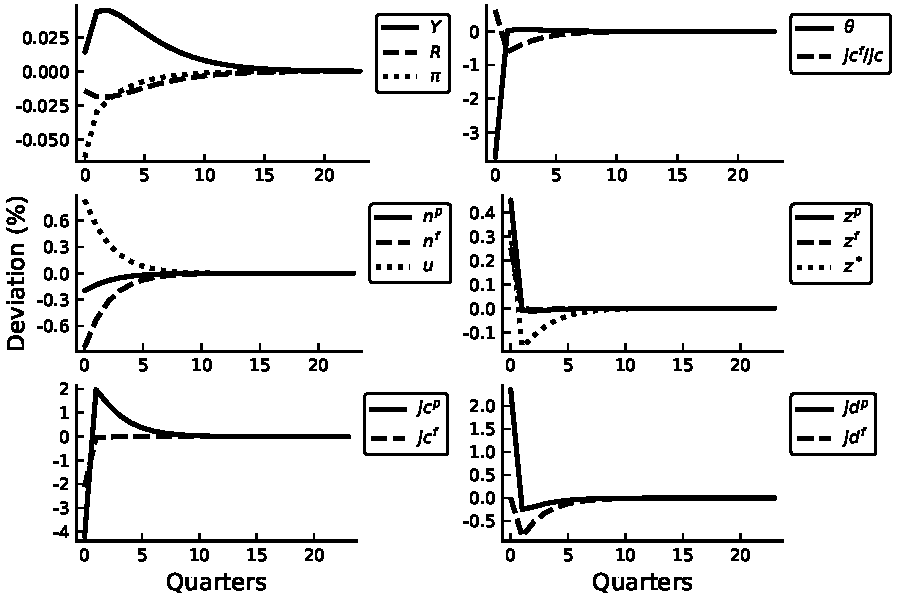
\includegraphics[scale=1]{irf_A.pdf}
\caption{IRF of main variables to a one-standard-deviation productivity shock}
\label{IRF_A}
\end{figure}

\paragraph{Productivity shocks} Figure \ref{IRF_A} displays the reaction of main variables to a productivity shock. An increase in labor productivity cuts real marginal costs. Inflation decreases and the central bank reduces nominal interest rates to encourage consumption. The support to demand is insufficient to prevent a decrease in employment. Unemployment increases while vacancies reduce, delineating a downward-sloping Beveridge curve and a decrease in labor market tightness. These results are classic in DSGE models with nominal rigidities. The downward sloping Beveridge curve is a traditional feature of Mortensen Pissarides models.

The behavior of flows constitute an important feature of labor markets. The enhanced productivity fuels higher job destruction among permanent contracts ; $z^p$ increases. Firms are more reluctant to keep low-productivity permanent matches as their expected gain from searching a worker enlarges. Job creation, as for it, immediately decreases through both permanent and temporary contracts because of of the drop in labor demand. Interestingly, job creation ends up increasing a few quarters after the observed cut on impact. This comes from a general equilibrium effect. Just after the shock, aggregate job destruction increases and job creation shrinks, which inflates the job seekers' pool for the next periods. This mechanically increases the subsequent job creation flows. On impact, output decreases because of the shrink in employment, which overcomes the productivity gains. Thereafter, the recovery of job creation pushes it up. 

The movements in thresholds $z^f$ and $z^*$ are key. The enhanced productivity makes firms' hiring policy more stringent and worker-firm pairs are more exacting about the productivity of an accepted match when they meet ; $z^f$ enlarges. The forces at stake when it comes to the evolution of $z^*$ are more complex. On one hand, the agents seek to benefit from productivity gains in full, which bolsters the attractiveness of permanent workers. On the other hand, firms are more demanding in terms of productivity when hiring a new permanent worker. On impact, the latter effect prevails, but it is quickly overcome by the former. The choice between a temporary and a permanent contract at the hiring stage also reflects the compromise between the fear of future rigidity and the appetite for productivity gains. Overall, productivity gains are insufficient to encourage substitution in favor of permanent contracts ; the transitory nature of the shock encourages the resort to temporary contracts, and the share of temporary contracts in job creation increases\footnote{This behavior stems from the location $z^f$ and $z^*$ occupy on the support of the distribution of idiosyncratic shocks, which Figure \ref{fig:pdf} shows. Movements in $z^f$ concern more formerly viable matches than similar movements in $z^*$, the slope of the probability density function of idiosyncratic shocks being higher in the neighborhood of $z^f$.}. Permanent employment unambiguously shrinks under the joint diminution in job creation and increase in job destruction. As for temporary contracts, job creation shrinks and job destruction occurs at a constant exogenous rate. Consequently, temporary employment decreases. 

\begin{figure}[t]
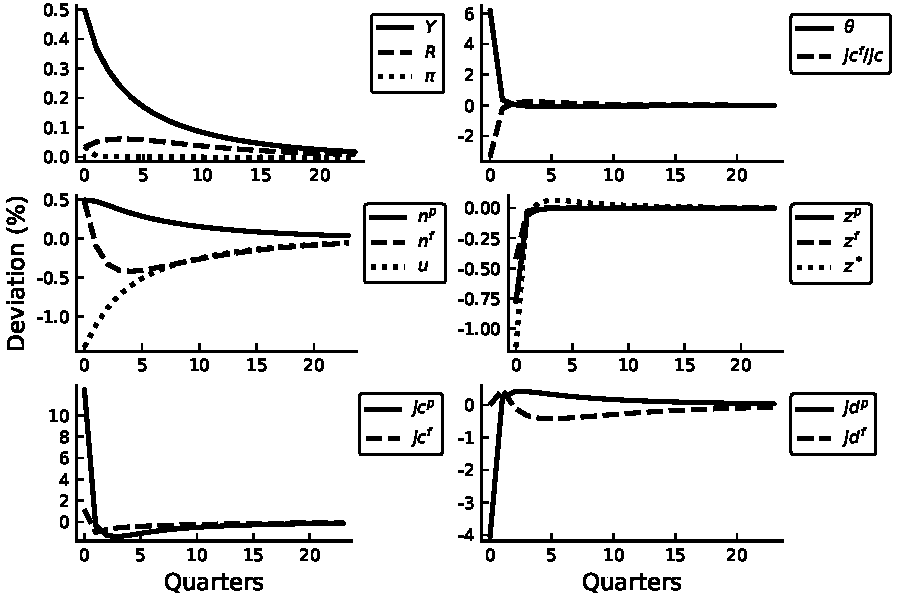
\includegraphics[scale=1]{irf_g.pdf}
\caption{IRF of main variables to a one-standard-deviation shock in government spending shock}
\label{IRF_g}
\end{figure}

\paragraph{Government spending shocks} Figure \ref{IRF_g} shows the impulse response functions of main variables after a shock in government spending. As usual in the literature, a sudden increase in government spending enhances output. Real marginal costs increase and the central bank increases the nominal interest rate to prevent the spread of inflation. The labor market tightness increases as firms post more vacancies to cope with the magnified demand of consumption goods. As a result, on impact, job destruction decreases and job creation increases. Interestingly, firms cope with the surplus of demand through an enlarged share of permanent contracts in job creation. The shock is persistent enough for the future expected losses associated with firing costs to be overcome by lifelong productivity gains. The general-equilibrium effect described in the preceding sections weighs in anew. Indeed, the shrink in the job seekers' stock exerts a downward pressure on job creations, which decrease below their steady-state values. While the transitional path of permanent employment remains above its steady-state value, temporary employment goes below its equilibrium level. As a matter of fact, fixed-term employment experiments a higher turnover, and is therefore highly impacted by temporary fluctuations in its associated job creation\footnote{This is all the more true since destruction rates of temporary jobs are constant}.

\begin{figure}[t]
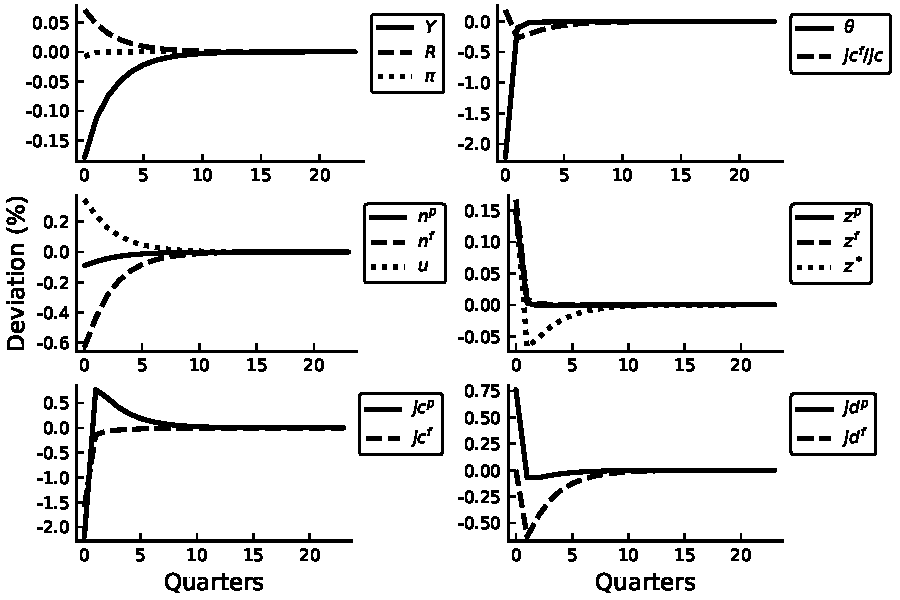
\includegraphics[scale=1]{irf_m.pdf}
\caption{IRF of main variables to a one-standard-deviation in the monetary policy shock}
\label{IRF_m}
\end{figure}

\paragraph{Monetary policy shock} Figure \ref{IRF_m} shows the impulse response functions of main variables after a shock in the monetary policy. A monetary policy shock pushes up interest rates, which discourages consumption and subsequently depresses output. Real marginal costs and inflation decrease. The marginal gross revenue from labor decreases and intermediate firms are overall more demanding in productivity terms to compensate the loss in profits ; firms post fewer vacancies and $z^p$ as well as $z^f$ increase. Thus, on impact, the labor market tightness shrinks and permanent job destruction enlarges. In turn, the formerly permanent employees join the ranks of the job seekers', which enhances job creation. Moreover, firms tend to switch to permanent contracts on behalf of temporary ones at the hiring stage in order to temper the immediate loss in revenue due to prices ; $z^*$ decreases. These two effects combined explain the observed rebound in permanent job creation.

As a result, viewed from the labor market, the monetary policy shock represents the negative of the government spending shock. The economic schemes at stake are the same. There is however a nuance. The effects of the monetary policy shock on the interest rate vanish much faster and the oscillations between the substitution effect and the general-equilibrium effect develop in a rougher way. This observation is also relevant when one considers the cost-push shock. The IRF of the latter will not be described, as it involves the same economic phenomena as the other shocks.

\subsection{Reforms in employment protection legislation}

In this paragraph, I examine the macroeconomic effects of a reform on employment protection legislation, which is summed up in firing costs here. I consider both transitory and permanent shocks. Transitory shocks are interesting, as employment protection legislation has frequently been the target of many reforms in Europe. \citet{fontaine2016cdd}, quoting a report from an observatory of the European Commission, mention the implementation of more than 220 policies related to employment protection legislation between 2005 and 2013. Permanent shocks, as for them, are relevant to study changes in volatilities of inflation, employment or output for example.

\begin{figure}[t]
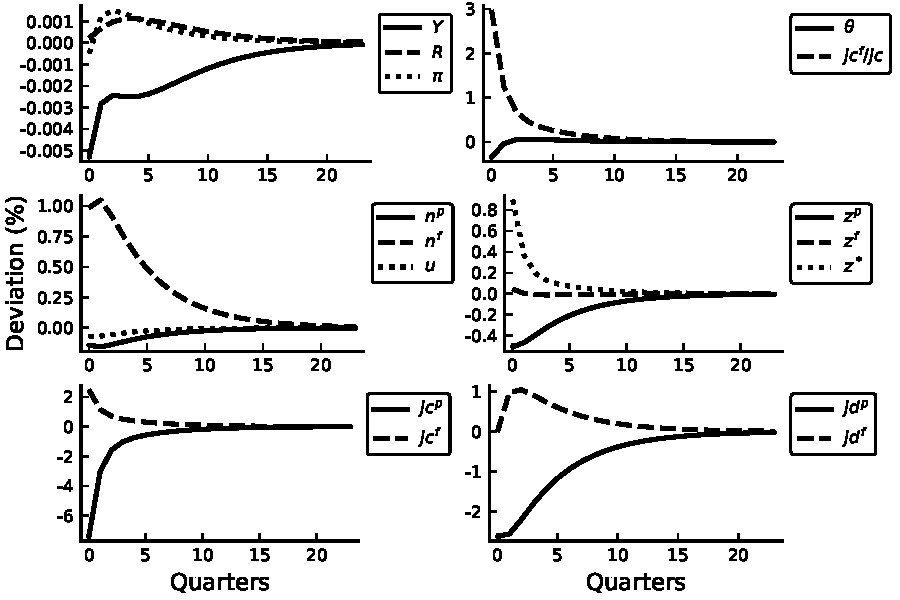
\includegraphics[scale=1]{irf_F.pdf}
\caption{IRF of main variables after a one-per-cent shock in firing costs}
\label{IRF_F}
\end{figure}

Figure \ref{IRF_F} displays the reaction of main variables to a one-percent positive shock to firing costs. The process for the logged shock is supposed to be an AR(1) with auto-regressive coefficient 0.8, so that the shock vanishes at 99\% five years after the impact. An increase in firing costs discourages job destruction ; $z^p$ and $jd^p$ decrease. Two opposite effects weigh on the composition of job creation. On one hand, enlarged firing costs entail costlier endogenous separations, which encourages substitution towards temporary job creation. On the other hand, these endogenous separations are scarcer. As a result, firms are less demanding in terms of productivity when it comes to hiring a permanent worker, which favors substitution towards permanent employment. In the present case, the former effect prevails ;  the share of temporary contracts in job creation increases.

Interestingly, the expected gain from posting a vacancy decreases because of the shrinking share of open-ended contracts in job creations. The resulting decrease in vacancy-filling rate joint with the tightened threshold for permanent hires reduces permanent job creation expands. The reduction in the permanent job destruction rate does no overcome the depleted permanent job creation rate and permanent employment dwindles. The substitution effect towards temporary contracts increases temporary job creation and temporary employment, as temporary job destruction occurs at a constant rate. Overall, output decreases. Inflation persistently increases in a hump-shaped manner even though the size of the response is small. Interestingly, a marginal and temporary change in firing costs generates long-lasting effects on inflation.

\begin{figure}[t]
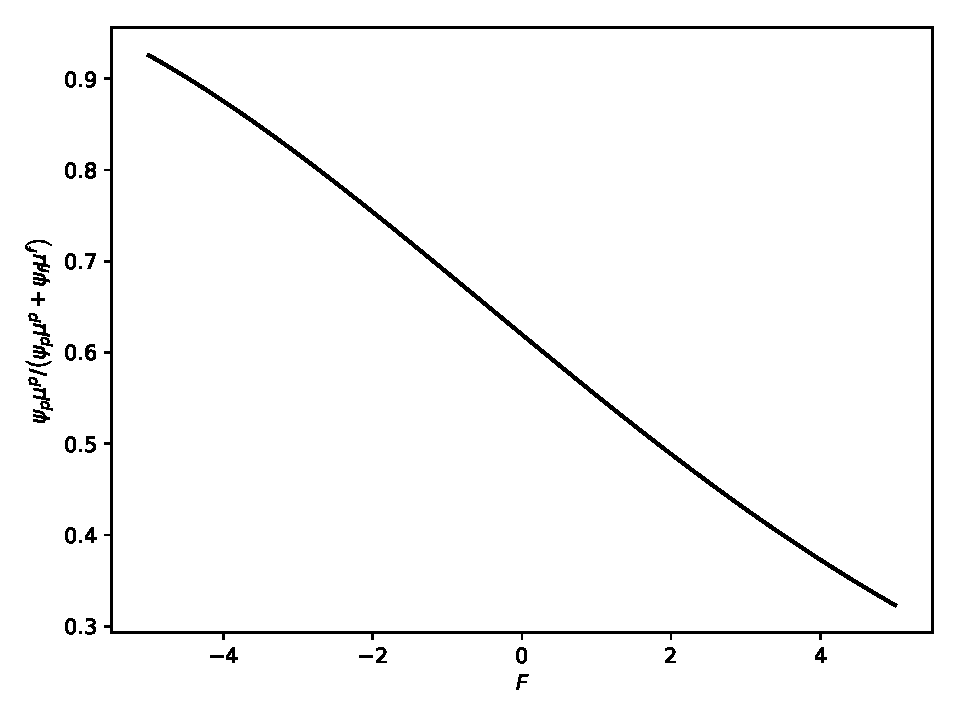
\includegraphics[scale=1]{NKPC.pdf}
\caption{The weight of permanent contracts in inflation dynamics in function of steady-state firing costs.}
\label{NKPC}
\footnotesize
\begin{flushleft}
The x-axis represents the percentage deviation of steady-state firing costs with respect to the baseline calibration, which is set at 0.
\end{flushleft}
\end{figure}


In order to understand the dynamics of inflation, I derive the New-Keynesian Phillips curve associated with the present model as is classic in the literature and find

\begin{align*}
\widehat{\pi_t} = \beta \mathbb{E}_t \widehat{\pi_{t+1}} + \kappa \left( \widehat{\mu_t} + \widehat{\phi_t} \right)
\end{align*}

where $\kappa = (1-\beta \psi) (1-\psi) / \psi$.

Meanwhile, I use the job creation condition to isolate $\phi_t$ and obtain

\begin{align*}
\phi_t = \frac{\gamma}{ (1-\eta) A_t \left[ \left( E_z \left[ z \middle| z \geq z_t^* \right] - z_t^c \right) q\left( \theta \right) \left( 1 - G\left( z_t^* \right)\right) + \rho \left( E_z \left[ z \middle| z_t^f \leq z \leq z_t^* \right] - z_t^f \right) q\left( \theta \right) \left( G\left( z_t^* \right) - G\left( z_t^f \right)\right) \right] }
\end{align*}  

The left-hand-side term in the bracketted part of the denominator is the expected surplus of production from a hire through permanent contract $\psi_t^p$ weighted with its probability of occurence $\mu_t^p$. This so-called surplus of production is the production of the match beyond the one corresponding to the zero-profit point. In an analogous manner, the right-hand-side term is the expected surplus of production from a hire through a temporary contract $\psi_t^f$ weighted by its probability of occurence $\mu_t^f$. Overall, the real marginal cost evolves negatively with the ability of the labor market to generate in expectations such production surpluses. This reminds the simple rule of a decreasing cost with respect to the abundance of a given good. Log-linearizing this condition and assuming that there are neither cost-push shocks nor productivity shocks, the New-Keynesian Phillips curve becomes

\begin{align*}
\widehat{\pi_t} = \beta \mathbb{E}_t \widehat{\pi_{t+1}} - \kappa \frac{\mu^p \psi^p}{\mu^p \psi^p + \mu^f \psi^f} \left( \widehat{\mu_t^p} + \widehat{\psi_t^p} \right) - \kappa \frac{\mu^f \psi^f}{\mu^p \psi^p + \mu^f \psi^f} \left( \widehat{\mu_t^f} + \widehat{\psi_t^f} \right)
\end{align*}

Retailers benefit from their market power and extract a rent from the production that exceeds intermediate firms' profitability thresholds. Interestingly, the discounted innovation in inflation is a weighted average, with the steady-state share of the newly hired workers' production for each contract as weights. The magnitude of these weights is difficult to assess, to the extent that they reflect a trade-off between a high hiring probability and a low average productivity, and conversely. The determinants of inflation dynamics are directly related to the evolution of the contractual composition of hires and their productivity. Figure \ref{NKPC} shows the importance of fluctuations on the permanent side of the labor market with different values of $F$, 0 being the baseline calibration. When $F$ increases, the weight of permanent contracts in the shaping of inflation dynamics decreases. As permanent job destruction becomes scarcer, the agents are less exacting in the productivity of hired permanent workers, which overcomes the enhanced permanent job creation ; the permanent side of the labor market loses importance when considering inflation dynamics. Importantly, these results highly depend on the distribution of idiosyncratic shocks. Nevertheless, as we changed $\sigma_z$ to 0.1 or 0.15, there were no notable difference in the results\footnote{An interval of values for the standard deviation of distribution of idiosyncratic productivity shocks $\sigma_z$ over which steady-state quantities are plausible is $( 0.1 , 0.22 )$}. Another important factor that influences inflation dynamics is the adjustment speed of employments, which is small in a labor market where flows are constrained by employment protection legislation. Consequently, reforms in employment protection legislation generate significant and persistent fluctuations in inflation. The size of the subsequent perturbations is small, though. A 10-per-cent cut in firing costs typically entails a 30-basis-point decrease in inflation on impact.